\documentclass[a4paper, 12pt]{article}
\usepackage{polski}
\usepackage{amssymb}
\usepackage[polish, english]{babel}
\usepackage[utf8]{inputenc}
\usepackage{mathtools}
\usepackage{amsthm}
\usepackage{amsfonts}
\usepackage{empheq}
\usepackage{xcolor}
\usepackage[pdftex,
            pdfauthor={Bartosz Sójka},
            pdftitle={Równoważność przez cięcia w przestrzeni dwuwymiarowej},
        %    pdfsubject={Równoważność przez cięcia w przestrzeni dwuwymiarowej}
            ]{hyperref}

%\setlength\parindent{0pt}

\newtheorem{observation}{Observation}[subsection]
\newtheorem{definition}[observation]{Definition}
\newtheorem{theorem}[observation]{Theorem}
\newtheorem{lemma}[observation]{Lemma}

\newcommand{\todo}[1]{\hfill \break \textbf{\Huge \textcolor{violet}{TO DO: #1} \hfill \break}\normalsize}
\newcommand{\content}[1]{\hfill \break \textbf{\large \textcolor{violet}{#1} \hfill \break}\normalsize}
\newcommand{\smalltodo}[1]{\textbf{\ \textcolor{violet}{To do}}}
\newcommand{\smalltodoII}[1]{\hfill \break \textbf{\ \textcolor{violet}{To do: #1}}\hfill \break}
\newcommand{\onedotsn}[1]{{#1}_1, \dots, {#1}_n}
\newcommand{\ndotsm}[3]{{#1}_{#2}, \dots, {#1}_{#3}}
\newcommand{\rysunek}[1]{\hfill \break\\[16pt] \Huge \textbf{\textcolor{violet}{Brakujący rysunek \normalsize
#1}} \hfill
\break \\[16pt] \normalsize}

\title{Równoważność przez cięcia w przestrzeni dwuwymiarowej}
\author{Bartosz Sójka}
%\date{}

\begin{document}
\thispagestyle{empty}
\begin{center}
\textbf{\large Uniwersytet Wrocławski\\
Wydział Matematyki i Informatyki\\
Instytut Matematyczny}\\
\textit{\large specjalność teoretyczna}\\
\vspace{4cm}
\textbf{\textit{\large Bartosz Sójka}\\
\vspace{0.5cm}
{\Large Równoważność przez cięcia w przestrzeni dwuwymiarowej}}\\
\end{center}
\vspace{3cm}
{\large \hspace*{6.5cm}Praca mam nadzieję magisterska\\
\hspace*{6.5cm}napisana pod kierunkiem\\
\hspace*{6.5cm}prof. dr. hab. Jana Dymary }\\
\vfill
\begin{center}
{\large Wrocław Rok 2019}\\
\end{center}
\newpage
\null
\thispagestyle{empty}
\newpage
\tableofcontents

\begin{abstract}
    W roku 1990 wegierski matematyk Miklós Laczkovich rozwiązał problem kwadratury koła Tarskiego - udowodnił
     on, że koło da się podzielić na skończoną liczbę części, z których można ułożyć kwadrat. Twierdzenie
     to może wydawać się nieintuicyjne i istotnie, części na które zostało podzielone koło w dowodzie były
     zbiorami niemieżalnymi, a sam dowód był niekonstruktywny. Co więcej, nie jest ono prawdziwe, gdy
     ograniczymy się do podziałów koła na zbiory, których brzegi są krzywymi Jordana. Punktem wyjścia
     pracy jest przypadek powyższego zagadnienia, gdzie brzegi są krzywymi Jordana kawałkami $C^\infty$.
     Można traktować je jako dobry model dla fizycznie realizowalnych cięć. Dalej będzie rozwinięta i
     omówiona teoria klasyfikacji figur w przestrzeni dwuwymiarowej ze względu na ich równoważność przez
     cięcia.
 \end{abstract}

 \section{Koło i kwadrat}
Praca będzie miała stopniowo rosnący poziom formalności. Początek jest gawędą o moich rozmyślaniach i
motywacjach skąd wzięły się przedstawione problemy. Mniej więcej między drugim a trzecim rozdziałem
całość nabiera formalizmu. Przez całą pracę rozważane krzywe są krzywymi sparamtryzowanymi długością,
 kawałkami $C^\infty$, gdzie kolejne $C^\infty$ fragmenty krzywych nigdy nie tworzą kąta $180 stopni$
 (tutaj formalniej). Będą one dalej nazywane po prostu krzywymi. \\
łuk - spójny fragment okręgu \\[16pt]
\includegraphics[width=\textwidth]{./rysunki/jpg/kolo_i_kwadrat.jpg} \\
Intuicja podwpowiada, że biorąc koło i tnąc je na skończenie wiele części nie dostaniemy takich, z których
da się ułożyć kwadrat. Co stoi za tą intuicją? Widać, że ewidentnym problemem jest brzeg koła, który jest
zaokraglony. Kwadrat żadnych zaokrągleń nie ma. Czy jednak aby na pewno to przeszkadza? Z pewnością, gdy
tniemy koło i dostaniemy kawałek, którego fragment brzegu jest fragmentem okręgu, to nie da się za pomocą
translacji i obrotów tego fragmentu odwzorować na fragment brzegu kwadratu. Jedno jest obłe, drugie jest
płaskie. Pojawia się jednak wątpliwość, czy jeśli potnie się koło na masę kawałków i część z tych kawałków
będzie miała odcinki jako krawędzie, które zostaną odwzorowane na brzeg kwadratu, to na przykłąd nie da się
tak wyciąćtych części, by "upchnąć" gdzieś również obłość okręgu. Przeciwko takiej możliwości świadczy
następujące rozumawanie. \\
Kiedy tnę figurę krzywą tak, żeby wprowadzić wklesłość, pojawia mi się również komplementarna do niej
wypukłość. \\
% \rysunek{}
\includegraphics[width=0.5\textwidth]{./rysunki/jpg/wkleslosc_wypuklosc.jpg} \\
Można spodziewać się więc, że próbując wyprodukować dla okręgu nadmiarową wklęsłość, starania te zawiodą,
gdyż za każdym razem powstanie tyle samo wypukłości. Tylko co to w tym wypadku znaczy "tyle samo"?
Nie wiedząc tego dalej pozostaje pewna wątpliwość, czy nie da się pociąć tak, by obłość zniknęła. widać, że
przy cięciach generujących wklęsłość obłość się pojawia, ale może pojawia się jej "mniej". Powinniśmy w takim
razie wprowadzić aparat pojęciowy pozwalający nam mierzyć "ilość" wklęsłości i obłości, tak by zobaczyć, czy
przy jakimkolwiek cięciu, da się wyprodukować jedno, nie produkujac jednakowej "ilości" drugiego. \\[4pt]
Przystąpimy do szukania satysfakcjonującej definicji obłości figury, która pozwoli nam rozróżnić
koło i kwadrat i sformalizować nasze intuicje. Obłość ma oddawać fakt, że coś jest zaokrąglone, więc dla bardziej
zaokrąglonych obiektów chcielibyśmy, żeby była większa, a dla mniej, żeby była mniejsza. Ponadto o obłości
figury ma świadczyć sam kształt brzegu danej figury. Zdefiniujmy zatem obłość dla krzywych. Powiemy, że
obłością figury z definicji jest tak zdefiniowana obłość jej brzegu. \\
Niech dowolnego odcinka jego obłość wynosi zero. Niech dla dowolnego okręgu jego obłość wynosi $2\pi$.
Niech dla spójnego fragmentu okregu jego obłość do obłości całego okręgu ma się tak jak jego długość do
długości całego okregu. Dzięki temu dla rodziny krzywych o tej samej długości $l$ - odcinka i fragmentów
okręgów wszystkich możliwych promieni ($[l/2\pi, \infty)$ faktycznie obłość jest tym większa im bardziej
zakrzywiona jest krzywa. \\
% \rysunek{}
\includegraphics[width=\textwidth]{./rysunki/jpg/coraz_bardziej_zakrzywione.jpg} \\
Zdefiniujmy teraz obłość dla krzywych $C^2$. \\
% \rysunek{ - podział krzywej, okręgi }
\includegraphics[width=\textwidth]{./rysunki/jpg/przyblizenia_okregami.jpg} \\
Definiujemy ją jako granicę przybliżeń obłości. \\
Przybliżamy obłość dzieląc krzywą na fragmenty i opisując okręgi tak jak na rysunku. Przybliżona obłość
fragmentu, to obłość odpowiadającego fragmentu okręgu. \\
Chcemy jednak rozróżniać "wklęsłość" od "wypukłości". Dlatego wybieramy stronę krzywej, która ma być
"wnętrzem" i sumujemy przyczynki z odpowiednimi znakami. \\

Granicą promieni okregów z kolejnyh przybliżeń w pojedynczym punkcie jest promień krzywej w danym punkcie.
Obłość dla łuku wyraża się jako długość przez promień. Skąd obłość krzywej jest całką po krzywej z
odwrotności promienia ze znakiem. Jest to więc całka po krzywej z jej krzywizny ze znakiem (oznaczanej
tutaj jako $k^\pm$. \\
% Teraz możemy wyrażać obłość liczbowo w upożadkowanym ciele liczb rzezywistych.
Zauważmy teraz, że cięcie figury nie zmienia jej obłości. Istotnie każda krzywa cięcia generuje dwie krzywe
brzegów fragmentów, które są identyczne z wnętrzmi po przeciwnych stronach. \\
Zatem całki ze znakowanej krzywizny (obłość) po nich są identyczne co do wartości i przeciwne co do znaku.
Zatem ich suma wynosi zero. \\
Stąd po poccięciu figura ma identyczną obłość, co przed. \\
Przesuwanie fragmentów i obracanie oczywiście nie zmienia obłości. Również klejenie fragmentóœ ze sobą nie
może jej zmienić, gdyż klejone fragmenty muszą być przystające i mieć wnętrze po przeciwnch stronach. Suma
ich obłości musi wynosić zatem zero. \\
Stąd operacja pocięcia na skończenie wiele fragmentów krzywymi i ponownego sklejenia nie zmienia obłości.
Koło ma jednak obłość rózną $2\pi$, a kwadrat równą $0$, zatem pocięcie w ten sposób jednego i sklejenie
drugiego jest niemożliwe.

\section{Pierścień i kwadrat}\label{ZMO}
Powyższe rozumowanie rozwiązuje problem dla koła i kwadratu, nie jest pomocne jednak w innym naturalnym
przykładzie, stworzonym wręcz po to (to prawda), żeby wykazać jego ograniczenia. \\
Weżmy pierścień i kwadrat. \\
% \rysunek{}
\includegraphics[width=\textwidth]{./rysunki/jpg/pierscien_kwadrat.jpg} \\
Intuicja, tak jak poprzednio, podpowiada nam, że nie powinno się dać jednego przekształcić na drugie
przy pomocy cięć i klejeń. Jednak obłość obydwu wynosi $0$.
Pierścień ma i wypukłości i wklęsłości, ale nie pasują one do siebie, więc spodziewamy się, że się nawzajem
nie "zniosą", jednak niezmiennik jakim jest obłość tego nie widzi. \\
Wyruszymy teraz na poszukiwania subtelniejszego niezmiennika, który wychwyci różnicę. Bedzie to
znakowana miara obłości. Ponownie zdefiniujemy ją dla krzywych z wyróżnioną stroną, a następnie
dla figur jako dziedziczoną z ich brzegu. \\
Jak widać problem leży w tym, że obłość wynosi zero, ale dodatnie i ujemne przyczynki pochadzą od okręgów
o różnych promieniach, które i tak do siebie nie pasują. Dlatego w dokładniejszym podejściu, rozróżniamy
od fragmentów krzywej o jakim proieniu pochodzi obłość. W tym celu definiujemy miarę, na przedziale
$\mathbb{R}$, równym $[0, K_\text{MAX}]$, gdzie $K_\text{MAX}$ jest maksymalną krzywizną występującą na
krzywej. Dla krzywej sparametryzowanej długością określamy ją jak następuje:
\begin{equation}
    \mu_O([k_1, k_2]) = \displaystyle\int\limits_{\{t\ :\ k(t) \in [k_1, k_2]\}}
    k^\pm\ \textrm{d}t.
\end{equation}
Tak zdefiniowana miara znowu jest niezmiennicza na cięcia (krzywe są identyczne, różnią się wyłącznie co do
strony wnętrza) jak i na izometrie zachowujące orientację i sklejenia. \\
Miara ta ma w każdym punkcie albo gęstość (gdy jakiś promień nie ma żadnego łuku), lub masę, gdy dany promień
 ma swój łuk. \\
 W przypadku pierścienia ZMO wynosi tyle: \\
 % \rysunek{}
 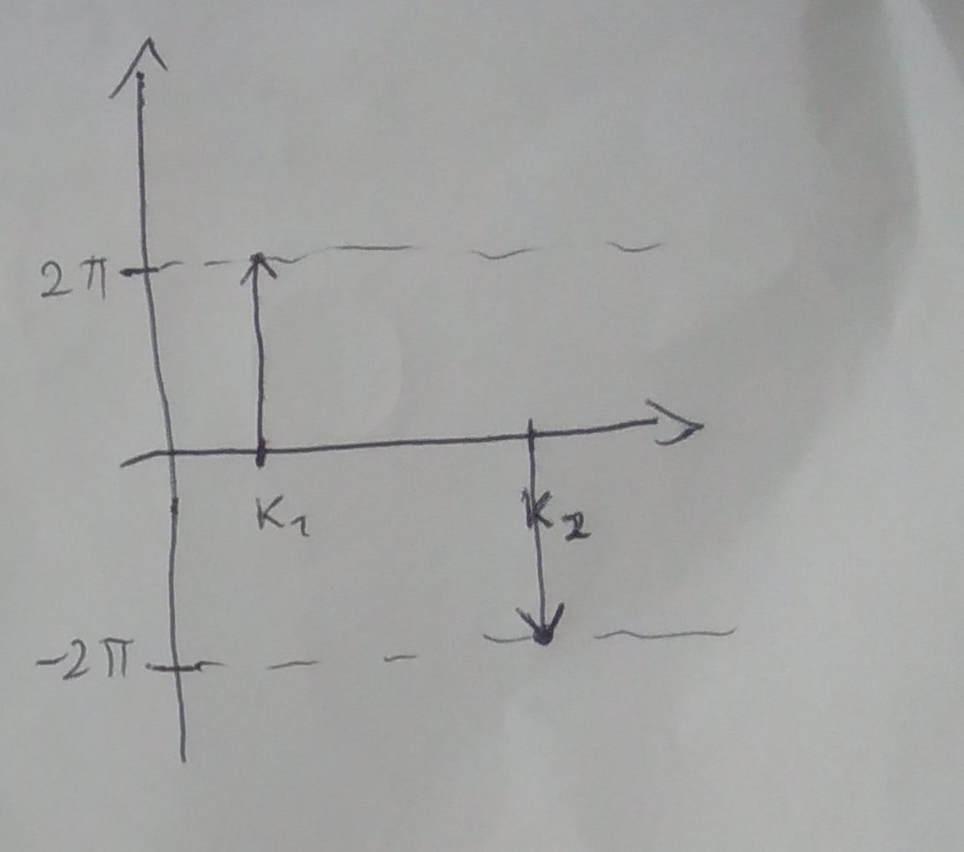
\includegraphics[width=0.5\textwidth]{./rysunki/jpg/zmo.jpg} \\
 W przypadku kwadratu wszędzie wynosi zero. \\
 Zatem faktycznie nie da się rozciać pierścienia i złożyć z niego kwadratu. \\

 Znakowana miara obłości pokrywa wszystkie naturalne przykłady (tzn. takie, które wymyśliłem, zanim starałem
 się wymysleć takie, które ją obalą). W szczególności potrafi nie tylko rozróżnić, ale i sklasyfikować
 wszystkie figury o brzegach składających się z odcinków i łuków (co pokażemy w następnym rozdziale). \\
 I tutaj zbliżamy się do prolemu - idealny niezmiennik pozwalałby nie tylko na określenie czy dla danych
 dwóch figur nie da się ich przerzucić. Wynikało by też z niego, że jeśli jest równy dla obu figur, to
 przerzucić się je da. Przy definiowaniu niezmienników jako własności brzegu wymaga to jednak chociażby
 faktu, że jeśli brzegi są sobie (w pewnym sensie jaki ściśle za niedługo podamy) równoważne przez cięcia,
 to figury także. Na szczęście okaże się, że tak jest. \\
 W kolejnych rozdziałach zajmiemy się własnie szukaniem takiego twierdzenia odwrotnego (czy właściwie
 działającego w obie strony) i związanego z nim niezmiennika. Zakończy się to dyskusją, czy wyniki nas
 satysfakcjonują. \\
 Pokażemy też w międzyczasie, że znakowana miara obłości takim niezmiennikiem nie jest (chociaż jest nim
 dla figur o brzegach składających się z odcinków i łuków).
 % Ale najpierw sformalizujmy nieco nasze pojęcia.
\section{Twierdzenie odwrotne}
Najpierw sformalizujmy nieco nasze pojęcia. \\
Zajmujemy się zwartymi figurami w $\mathbb{R}^2$, których brzegi są skończonymi zbiorami rozłącznych obrazów
prostych krzywych
zamkniętych, kawałkami $C^\infty$, takimi, że, żadne dwa sąsiednie $C^\infty$
kawałki obrazów jednej krzywej
nie tworzą ze sobą kąta $180 stopni$. Co to znaczy, że nie tworzą kąta $180 stopni$? O to: \\
% \rysunek{}
\includegraphics[width=0.5\textwidth]{./rysunki/jpg/180_stopni.jpg} \\
i wyjaśnienie \\

Wszędzie dalej kiedy będzie użyte słowo figura, będzie to oznaczało właśnie taki podzbiór $\mathbb{R}^2$. \\
Ponadto wszystki krzywe parametryzujemy ich długością.
\subsubsection{Krzywa z wyróżnioną stroną}
Krzywa z wyróżnioną stroną będzie to krzywa wraz z wybraną jedną z dwóch klas ciągłych cięć pewnej wybranej
 podwiązki wiązki stycznej $\mathbb{R}^2$ zawieszonej nad tą krzywą. \\
Dla krzywej $\gamma : [a, b] \to \mathbb{R}^2$ patrzymy się na podwiązkę wiązki stycznej do
$\mathbb{R}^2$ złożoną
z dowolnych podprzestrzeni dopełniczych do podprzestrzeni rozpinanych przez wektor styczny do krzywej w
danym punkcie. (na rogach wybieramy tak, by przestrzeń była dopełnicza dla obu wektorów stycznych). \\
Wybieramy teraz ciągłe, nieznikające cięcia tych wiązek, takich, aby w punktach nieróżniczkowalności
wyznacznik macierzy złożonej z wybranego wektora i z wektora stycznego miał taki sam znak dla obydwu
wektorów stycznych. \\
% \rysunek{}
\includegraphics[width=\textwidth]{./rysunki/jpg/w_te_sama_strone.jpg} \\
\smalltodoII{Może ująć to w lemat:}
Dzielą się one na dwie klasy: \\
-cięcia, gdzie w każdym punkcie wyznacznik macierzy [wektor styczny, wektor z cięcia] jest dodatni oraz\\
-cięcia, gdzie w każdym punkcie wyznacznik macierzy [wektor styczny, wektor z cięcia] jest ujemny \\
Jest tak, ponieważ cięcia te są ciągłymi cięciami jednowymiarowej wiązki, wyznacznik jest ciągły oraz
zależność wektora stycznego od parametru jest ciągła poza punktami nieróżniczkowalności, ale na nich,
z wyboru wiązek, wyznacznik nie zmiania znaku. Stąd wyznacznik musiałby zmieniać znak we wnętrzu
różniczkowalnej krzywej, ale wtedy w pewnym momencie zerowałby się, co oznaczałoby, że cięcie znika.
Sprzeczność. \\
Wybór jednej z klas takich cięć nazywamy wyborem strony krzywej. Ma to oddawać fakt czegoś takiego: \\
% \rysunek{}
\includegraphics[width=0.5\textwidth, angle=90]{./rysunki/jpg/ma_oddawac_cos_takiego.jpg}
Zauważmy, że dla figury rozpatrywanej jako dwuwymiarowa rozmaitość oraz komponenty jej brzegu jedna z tych
klas jest złożona z wektorów leżacych w wiązce stycznej do tej rozmaitości, a jedna z wektorów do niej
nienależących. Ponieważ dla każdej komponenty parametryzację możemy wybrać niezależnie, więc da się je wybrać
tak, by jedna z tych klas odpowiadała dla wszsytkich komponent wnętrzu rozmaitości. Od tej pory będziemy
zakładali taki właśnie wybór parametryzacji. Co więcej taki, by strona z ujemnym wyznaczniekiem była we
wnętrzu.
% (Czyli obiegamy figury przeciwnie do ruchu wskazówek zegra).
\\

Od tej pory o wszystkich krzywych zakładamy, że mają wyróżnioną stronę.
Krzywiznę ze znakiem $k^\pm$ określamy tak, że jeśli para: wektor styczny, wektor drugiej pochodnej ma ten
sam znak co wybrana klasa, to $k^\pm = k$, w przeciwnym wypadku $k^\pm = -k$.
\subsection{Równoważność z problemem na brzegach}
Najpierw dowiedziemy, że zagadnienie równoważności takich figur przez cięcia jest równoważne równoważności
przez cięcia ich brzegów w następujacym sensie: \\
Powiemy, że dwie krzywe są równoważne przez cięcia, jeżeli obraz jednej z nich można pociąć i za pomocą
izometrii zachowujących orientację przekształcić na obraz drugiej (zachowując wyróżnioną stronę), przy czym dopuszczamy cięcia pustej
przestrzeni na dwie
odpowiadające sobie krzywe oraz sklejanie takich krzywych: \\
% \rysunek{słynne rysunki rozcinania pustej przestrzeni oraz klejenia dwóch odpowiadających krzywych
% dopiski - kreacja, anihilacja}
\includegraphics[width=\textwidth]{./rysunki/jpg/kreacja.jpg} \\
\includegraphics[width=\textwidth]{./rysunki/jpg/anihilacja.jpg} \\
W jedną stronę: \\
jeśli da się przerzucić brzegi na siebie, a figury mają równe pola, to da się również figury. \\
Weźmy dwie figury $A$ oraz $B$ o równych polach, takie, że brzegi są równoważne przez cięcia. Niech cięcie
to będzie realizowane poprzez podział brzegu $A$ i przekształcenie jego fragmentów przez przesunięcia
i obroty oraz,
jeśli konieczny, podział "pustej przestrzeni" na krzywe i anihilację pasujących krzywych tak jak opisane
wyżej. Niech ta operacja świadcząca o równoważności dwóch brzegóœ przez cięcia nazywa się $\phi$ \\
Skonstruujemy teraz redukcję problemu podziału tych figur do problemu podziału wielokątów, który, jak wiadomo
 z Wallace–Bolyai–Gerwien theorem, zawsze ma rozwiązanie. \\
Rozpatrzmy fragmenty na które podzielony jest brzeg $A$. Każdy z nich jest zbiorem zwartym, więc
(za wyjątkiem sąsiadujących) jest on w niezerowej odległości od pozostałych fragmentów. Dla tych, których
 obraz przez $\phi$ jest w $B$ (to znaczy, że fragment nie został zanihilowany z mu odpowiadającym)
 jest on również w niezerowej odległości od wszystkich fragmentów (za wyjątkiem tych z którymi ma wspólne
 końce) z których został ułożony brzg $B$ przy  użyciu $\phi$.  \\
Fragmentów jest skończenie wiele, niech więc $\varepsilon$ będzie dodatanią liczbą rzeczywistą mniejszą
od wszystkich tych odległości dla wszystkich par niesąsiadujących fragmentów. \\
rozpatrzmy $\frac{\varepsilon}{4}$-owe otoczki wszystkich fragmentów krzywej. W każdym z tych fragmentów
prowadzimy
łamaną prostą o początku i końcu w końcach fragmentu taką, że piersza i ostatnia krawędź łamanej
\label{180 stopni} spełnia
następujący warunek na kąty względem wektorów stycznych (zarówno w $A$, jak i w $B$: \\
% \rysunek{początek i koniec łamanej, dwusieczna kąta  z wektorów stycznych}
\includegraphics[width=\textwidth]{./rysunki/jpg/konce_lamanej.jpg} \\ % poczatek i koniec lamanej
% \rysunek{przypadek 180 stopni}
Wtedy wszystkie obszary ograniczone przez fragmenty krzywej oraz łamane w odpowiadających im
otoczkach oraz ich obrazy prze $\phi$ są parami rozłączne za wyjątkiem końców fragmentów dla
sąsiadujących fragmentów. \\
Możemy odciąć je z $A$ i przerzucić w odpowiednie miejsca na $B$. \\
Fragmenty brzegu $A$, które się z sobą zanihilują, odcinamy po jednym z pary wraz z jego łamaną i
anihilujemy. \\
% \rysunek{anihilecja}
\includegraphics[width=\textwidth]{./rysunki/jpg/przeksztalcenie_A_A'.jpg} \\
Niech $A'$ oznacza tak powstałą z $A$ figurę.
Brzeg $B$ dzieli się na dwa obszary - fragmenty pochodzące z fragmentów brzegu $A$ oraz fragmenty
pochodzące z rozcięć przestrzeni.
Pozostaje "obsłużyć" fragmety brzegu $B$ pochadzące z kreacji krzywych z przestrzeni. \\
Potrzebny będzie następujący lemat:
\begin{lemma}\label{lemat o dzieleniu}
    Dla dowolnej krzywej $\gamma : [a, b] \to \mathbb{R}$ takiej jak tu przyjmujemy i dowolnego okręgu
    $\mathcal{O}$ zawartego w $\mathbb{R}^2$ da się znaleźć taki podział $\gamma$, by poprzez
    przesunięcia i obroty
    dało się go odwzorować we wnętrze $\mathcal{O}$ tak, że obrazy fragmentów są parami rozłączne.
\end{lemma}
\begin{proof}
    % Obłość $\gamma$ jest skończona, zatem skończona jest obłość każdego fragmentu $\gamma$.
    Konstuujemy ciąg podziałów $\gamma$
     tak, by dla każdego $n$ w $n$-tym podziale
     % obłość kazdego fragmentu była mniejsza niż $\pi/2^n$ oraz by
     długość każdego fragmentu była mniejsza niż $d(\mathcal{O})/(2n+1)$ ale (poza, być może, ostatnim)
      większa niż $d(\mathcal{O})/(2n+3)$. \\
      \smalltodoII{dać lepsze oznaczenia}
     Fragmentów tych będzie co najwyżej część całkowita z $\frac{d(\gamma)}{d(\mathcal{O})/(2n+3)}$.
     czyli $(2n+3)\frac{d(\gamma)}{d(\mathcal{O})}$. Każdy z tych fragmentów zmieści się w kole
     o średnicy $d(\mathcal{O})/(2n+1)$. Kół o średnicach $d(\mathcal{O})/(2n+1)$ w kole $\mathcal{O}$ da się
      na pewno zmieścić co najmniej $6\frac{n(n+1)}{2}+1$. \\
      % \rysunek{sześciokąty}
      \includegraphics[width=\textwidth]{./rysunki/jpg/szesciokaty.jpg} \\
      Dla $n$ takiego że $3\frac{n(n+1)+1}{2n+3}>\frac{d(\gamma)}{d(\mathcal{O})}$, krzywa zmieści się
      rozłącznie w okręgu dla podziału odpowiadającego $n$.
     % \begin{lemma}
     %     Dla każdego takiego podziału krzywa zmieści się w kole o promieniu $a$.
     % \end{lemma}
     % \begin{proof}
     %
     % \end{proof}
\end{proof}

Bierzemy wszystkie krzywe (bez wyróżnionej strony) z których powstały te fragmenty brzegu $B$, łączymy je
w jedną długą krzywą prostą (jeśli trzeba to łamiemy je, żeby zachować warunek "prostości").
Tak skonstruowaną krzywą umieszczamy w kole tak małym, by było zawarte we wnętrzu $A'$ tak jak mówi lemat
\ref{lemat o dzieleniu}. \\
\includegraphics[width=\textwidth]{./rysunki/jpg/krzywa_w_szesciokacie.jpg} \\
Przy czym zagęszczamy podział tak mocno by obłość każdego fragmentu nie
przekraczała $\pi/8$ oraz by dlugość żadnego fragmentu nie była większa niż $\varepsilon/8$. \\
Należy teraz wykonać następujące cięcia w $A'$: \\
% \rysunek{jak ciąć}
\includegraphics[width=\textwidth]{./rysunki/jpg/jak_ciac.jpg} \\
% \rysunek{jak ciąć w środku kulki}

Z powyższych fragmentów układamy odpowiednie fragmenty brzegu $B$. \\
Tak powstała figura $A''$ jest wielokątem. Niepokryta część $B$ rówież jest wielokątem,
nazwijmy ją $B''$. $A$ oraz $B$ miały równe pola, więc $A''$ i $B''$ również mają równe pola.
Są więc równoważne przez cięcia, więc $A$ i $B$ również są. \\[8pt]

W drugą stronę: \\
Jeśli figury są równoważne, to brzegi też. \\
Podział figur zadaje równoważność brzegu jednej z sumą brzegów fragmentów na jakie została pocięta
oraz równoważność tej sumy brzegów z brzeiem drugiej. Stąd dla równoważnych figur ich brzegi również są
równoważne.
$_\square$ \\
\textbf{Uwaga.} To właśnie w tym dowodzie potrzebne jest założenie, że fragmety krzywych nie mogą tworzyć
kątu 180 stopni. Konkretnie w \hyperref[180 stopni]{tym}. W przypadku 180 stopni nie dałoby się skonstruować
odpowiednich łamanych. \\
Przykładem figury której brzeg jest równoważny przez cięcia z brzegiem innej, o równym polu, a które nie
spełniają jedynie tego założenia i nie są równoważne przez cięcia są następujące figury: \\
% \rysunek{posklejane kółka ze szpicami}. \\
\includegraphics[width=0.5\textwidth]{./rysunki/jpg/szpice_pierscien.jpg} \\
 \includegraphics[width=\textwidth]{./rysunki/jpg/kolo_ze_szpicami.jpg} \\
\text{Dowód nierównoważności:} \\
\todo{jakiś niezmiennik na szpice, to powinno wyjść}

\subsection{Kiedy ZMO zawodzi}
Pokazaliśmy, że rozstrzygając równoważność przez podział figur o tym samym polu wystarczy roztrzygnąć
równoważność przez podział ich brzegów. Zastanówmy się, czy znakowana miara obłości jest wystarczającym
kryterium do klasyfikacji krzywych - tzn. czy dowolne dwie nierównoważne mają różną oraz czy dowolne
dwie równoważne mają taką samą. \\
W \ref{ZMO} odpowiedzieliśmy sobie twierdząco na drugie pytanie.
% Pokażemy teraz, że odpowiedź na pierwsze
% pytanie jest twierdząca dla krzywych złożonych wyłącznie z łuków i odcinków.
Odpowiedź na pierwsze pytanie jest twierdząca dla krzywych złożonych wyłącznie z łuków i odcinków.
Mając tą samą znakowaną miarę obłości mają tą samą sumaryczną długość łuków okręgów o odpowiednich
promieniach z wyróżnioną stroną z odpowiedniej strony. Fragmenty te można kleić ze sobą i ciąć, tak by
z jednej krzywej otrzymać drugą. Fragmenty o krzywiźnie 0 można dowolnie kreować i anihilować. \\
Znakowana miara obłości nie potrafi jednak rozróżnić wszystkich nieprzystających do siebie przez cięcia
krzywych. Skonstruujemy tego przykład. Najpierw jednak przeprowadzimy analizę czym jest
wprowadzona tutaj znakowana miara obłości i jak ma się do krzywizny krzywej.
\subsubsection{Jak wygląda znakowana miara obłości}
Rozpatrzmy krzywą o ściśle monotonicznej krzywiźnie.
Dla takich krzywych znak znakowanej krzywizny jest stały. Rozpatrzmy najpierw przypadek, gdzie $k^\pm = k$.
\\
 Niech $k(t)$ będzie funkcją krzywizny od czasu jakim
jest
sparametryzowana. Ze ścisłej monotoniczności istnieje funkcja odwrotna $t(k) : [k_\text{MIN}, k_\text{MAX}]
\to \mathbb{R}$, która mówi w jakiej chwili czasu uzyskana była dana wartość krzywizny. \\
Wyrazimy teraz znakowaną miarę obłości takiej krzywej poprzez jej krzywiznę oraz na odwrót - jej krzywiznę
poprzez jej znakowaną miarę obłości. \\
\begin{lemma}
    Dla krzywej o ściśle rosnącej krzywiźnie jej ZMO ma gęstość.
\end{lemma}
\begin{proof}
    Z definicji znakowanej miary obłości, dla dowolnego przedziału $[k_1, k_2]$ jest ona równa:
    \begin{equation}
        \mu_K([k_1, k_2]) = \displaystyle\int\limits_{t(k_1)}^{t(k_2)}k(t)\ \text{d}t
    \end{equation}
    Co przez zamianę zmiennych jest równe:
    \begin{equation}
        \displaystyle\int\limits_{t(k_1)}^{t(k_2)}k(t)\ \text{d}t =
        \displaystyle\int\limits_{k_1}^{k_2}\frac{k}{k'(t(k))}\ \text{d}k
    \end{equation}
    $\varrho_K(k) = \frac{k}{k'(t(k))}$ jest szukaną gęstością miary $\mu_K$.
\end{proof}
W ten sposób dla takiej klasy krzywych wyraziliśmy gęstość ich ZMO poprzez ich krzywiznę. Dla krzywych bez
łuków $\mu_K$ rownież ma gęstość, jest ona wtedy sumą gęstości jej składowych o ściśle monotonicznej
krzywiźnie.
Jest tak ponieważ definiujemy tę miarę poprzez całkę, która jest operatorem liniowym. \\
\smalltodoII{określić jakie trzeba przyjąć warunki początkowe}
Możemy wyrazić krzywiznę krzywej o ściśle monotonicznej krzywiźnie na podstawie jej ZMO rozwiązując równanie
różniczkowe:
\begin{equation}
    \varrho_K(t) = \frac{k(t)}{k'(t)}
\end{equation}
Jego rozwiązaniem jest:
\begin{equation}
    k(t) = k_0e^{\int_{t(k_0)}^{t}\frac{1}{\varrho_K(w)}\text{d}w}
\end{equation}
Gdzie $k_0$ to odpowiednio najmniejsza bądź największa krzywizna. \\
Dla przypadku, gdzie $k^\pm = -k$ otrzymane zależności to:
\begin{align}
    \varrho_K(k) &= -\frac{k}{k'(t(k))}\ \
    % \varrho_K(t) &= -\frac{k(t)}{k'(t)}\
    \textrm{oraz} \\
    k(t) &= k_0e^{\int_{t(k_0)}^{t}-\frac{1}{\varrho_K(w)}\text{d}w}.
\end{align}
Jako, że w obydwu przypadkach znakowana krzywizna ma stały znak, możemy odtworzyć również wyróżnioną stronę
krzywej - w pierwszym przypadku jest to strona której reprezentantem są wektory II pochodnej. W drugim
przpadku - wektory do nich przeciwne. \\

\subsection{No i co z tego?}
Krzywa będąca konkatenają dwóch krzywych o ściśle rosnącej krzywiźnie o mierze obłości: \\
% \rysunek{}
\includegraphics[width=0.5\textwidth]{./rysunki/jpg/polowkowa_krzywizna.jpg} \\
każda. Ma tą samą miarę obłości co krzywa o ściśle rosnącej krzywiźnie i mierze obłości: \\
% \rysunek{}
\includegraphics[width=0.5\textwidth]{./rysunki/jpg/calkowita_krzywizna.jpg} \\
Nie są one jednak równoważne przez cięcia. Dla dowolnej ustalonej wartości krzywizny mają one bowiem różne
wartości pochodnej tej krzywizny. \smalltodoII{napisać dokładniej czemu}.
By potrafić odróżnić od siebie istotnie różne krzywe potrzebujemy niezmiennika zawierającego w sobie
informacje o parametryzacji. Należałoby zawrzeć jakoś informacje jak krzywa rozkłąda się na krzywe o ściśle
monotonicznej krzywiźnie, które już są wyznaczone jednoznacznie (z dokładnością do przesunięć i
obrotów) przez ich ZMO.
Wtedy znalibyśmy rodzinę krzywych z dokładnością do ich cięć i przesunięć oraz obrotów.
W następnym rozdziale przedstawimy niezmiennik, który faktycznie jest zachowywany przy cięciach
przesunięciach oraz obrotach i
 sklejeniach oraz jest różny dla krzywych (a stąd dla figur) które równoważne nie są.

\section{Wielka grupa abelowa}
Niech $\mathcal{A}$ będzie rodziną wszytkich
prostych krzywych
zamkniętych, kawałkami $C^\infty$, takimi, że, żadne dwa sąsiednie $C^\infty$ kawałki obrazów jednej krzywej
nie tworzą ze sobą kąta $180 stopni$, sparametryzowanych długością z wyróżnioną stroną
(zapisywaną jako $\mathcal{S}(\gamma) = 1$ bądź $\mathcal{S}(\gamma)=-1$. \\
Rozepnijmy wolna grupę abelową na $\mathcal{A}$. \\
Określmy teraz relacje w tej grupie: \\
-kreacji/anihilacji \\
-cięcia/klejenia \\
-izometrii zachowujących orientację \\

\subsubsection{Kreacja/anihilacja}
Dla $\gamma_1 : [a, b] \to \mathbb{R}^2, \gamma_2 : [c, d] \to \mathbb{R}^2$
\begin{gather}
    \Big( \gamma_1[[a,b]]=\gamma_2[[c,d]] \\\land\\
    \big( (\gamma_1(a) = \gamma_2(c) \land \mathcal{S}(\gamma_1)=\mathcal{S}(\gamma_2)\big) \\\lor \\
    \big(\gamma_1(a) = \gamma_2(d) \land \mathcal{S}(\gamma_1)\neq\mathcal{S}(\gamma_2)) \big) \Big)\\
     \implies \gamma_1 + \gamma_2 = 0
\end{gather}
\subsubsection{Cięcia/klejenie}
Dla $\gamma_0 : [a_1, a_n] \to \mathbb{R}^2, \gamma_1 : [a_1, a_2] \to \mathbb{R}^2, \ldots, \gamma_n :
[a_{n-1}, a_n] \to \mathbb{R}^2$, takich że $a_1 < a_2 < \ldots < a_{n-1} < a_n$
\begin{gather}
    \Big(
    (\forall t \in [a_i, a_{i+1}])(\gamma_0(t)=\gamma_i(t)) \land (\forall i)\mathcal{S}(\gamma_0) =
    \mathcal{S}(\gamma_i)
    \Big) \\
    \implies \gamma_0 - \gamma_1 - \ldots -\gamma_n = 0
\end{gather}
\subsubsection{Izometrie zachowujące orientacje}
Dla $\gamma_1 : [a, b] \to \mathbb{R}^2, \gamma_2 : [c, d] \to \mathbb{R}^2$
\begin{gather}
    ( k^\pm(\gamma_1) \equiv k^\pm(\gamma_2)
    \land
    \mathcal{S}(\gamma_1)=\mathcal{S}(\gamma_2))
    \implies \gamma_1 - \gamma_2 = 0
\end{gather}
Odpowiada to odwzorowaniom przez izometrie zachowujące orientację $\mathbb{R}^2$.
\begin{gather}
    (\exists\Lambda_{-\text{izometria}}\ \gamma_1 \equiv \Lambda\circ\gamma_2
    \land \mathcal{S}(\gamma_1)=\mathcal{S}(\gamma_2))\implies \gamma_1 - \gamma_2 = 0
\end{gather}
ponieważ funkcja znakowanej krzywizny określa jednoznacznie krzywą (bez wyróżnionej strony)
z dokładnością do jej początku i wektora stycznego w początku.
\smalltodoII{napisać równanie różniczkowe}
Druga pochdna równa się wektor prostopadły do pierwszej dodatnio zorintowany razy znakowana krzywizna. \\
\begin{equation}
    (\gamma''_x, \gamma''_y)(t) = k^\pm(t)(-\gamma'_y, \gamma'_x)(t)
\end{equation}
\smalltodoII{napisać coś o rozwiązaniu tego równania}

Zauważmy, że trzecia relacja utożsamia również krzywe o tym samym obrazie, a różnej parametryzacji ze
względu na przedział którym są sparametryzowane.
\section{Równoważność elementu w wielkiej grupie abelowej z klasą figur równoważnych ze sobą przez cięcia}
Widać \\
W jedną stronę - weźmy element z WGA, pokażemy, że odpowiadamu dokładnie jedna klasa równoważności krzywych.
\\
Jeśli odpowiadałyby dwie, to biorę po reprezentancie każdej z nich i patrzę na ich elementy w niewydzielonej
grupie, są tym samym w wydzielonej, więc te relacje jakoś je zwijają. \\
To generuje cięcia. \\
% To senioeoofaja cięcoa. {onadfoeofe możena z zauważeć , zę w pownem momecicie zacząłem pisać całkowicie verz
% patrzenia na klawoateurę
% po odzie rto znacznoe lieoaj nież się zspodzieawałem. zSz czełdó lnei ż e staeałen się apasiasć wiraen sirwas
%  sdioasgsi c szir czo0od aifa naiej fpsijiakdf/ nke.
Jeśli dwie figury są w tej samej klasie, to są te transformacje, które o tym świadczą, przenossą się one na
grupę. \\
\section{Dyskusja, że to niewiele daje}
Niezmiennik jakim jest element w WGA faktycznie daje charakteryzaję. Jednak jego wyznaczenie (bądź w ogóle
opisanie) nie wydaje się łatwiesze niż rozstrzygnięcie problemu dla danych figur bez tego aparatu
pojęciowego. Wiedza o możliwości przedstawienia tego problemu w postaci WGA nie dała mi żadnej odpowiedzi
na żadne pytanie postaci "opisuję jakoś dwie figury, chcę rozstrzygnąć, czy są równoważne przez cięcia",
którego nie potrafiłbym rozstrzygnąć w iinny sposób. Opis ten daje jednak inne rzeczy.\\
Odzwierciedliliśmy bowiem problem w strukturę grupową. Zrobiliśmy to również w taki sposób, że każdej klasie
figur równoważnych przez cięcia odpowiada jeden element w grupie abelowej oraz liczba rzeczywista (pole)
oraz każdemu elementowi z grupy wraz z liczbą z zakresu $(0, \infty)$ (możliwe pola, bo tnąc zawsze można
zejść dowaolnie blisko zera "redukując kąt zataczany przez krzywe i zbliżając powstałe krawędzie", a
kreując krzywe można uzyskać dla wybranej klasy dowolnie duże pole). \\
% \rysunek{redukcja krzywizny}
\includegraphics[width=\textwidth]{./rysunki/jpg/IMG_20190902_162303.jpg} \\
odpowiada jedna klasa figur równoważnych przez podział. \\
Załóżmy teraz, ze chcemy okreslić pewien niezmiennik, prostszy w wyliczeniu, ale taki, że jego możliwe wyniki
nadal będą w bijekcji z klasami podziału. Załóżmy ponadto, że przeciwdziedzina tego niezmiennika będzie miała
strukturę grupową. Jest to dość naturalne założenie, pierwsze dwa naturalne niezmienniki jakie wprowadziliśmy
, mianowicie obłość i znakowana miara obłości, miały tę strukturę, a niezmienniki były homomorfizmami,
gdzie po jednej stronie działaniem było wzięcie na raz dwóch krzywych (albo, można myśleć ich konkatenacja),
a po drugiej stronie - suma ich niezmienników. \\
Wydaje się, że jeśli niezmiennik wyrażony w czymś o strukturze grupowej miałby się zachowywać "przyzwoicie"
powinien mieć tę własność. Mając jednak naszą WGA widzimy, że każdy taki niezmiennik pozwalający na
rozróznianie dwóch dowolnych klas oraz nie mający będzie miał zanurzoną w sobie WGA, w tym sensie będzie
nieprostszy. \\
Oczywiście nie wykluczam, że nie spostrzegłem jaki metod rozróżniania klas figur przy użyciu innego typu
niezmienników bądź bez określania niezmienników wgl. Może też istnieje efektywna metoda określania
jednakowości elementóœ w WGA. Jednak na ten moment żadne z powyższych nie zostało przeze mnie znalezione.
% pewnego zakresu charakterystycznego dla tego elementu (możliwe pola)
\section{a co, jeśli, krzywe są zamknięte i (nie kawałkami!) głądkie?}
\includegraphics[width=0.25\textwidth]{./rysunki/me_whenjpg.jpg}
\includegraphics[width=0.25\textwidth]{./rysunki/me_skletonjpg.jpg}
\includegraphics[width=0.25\textwidth]{./rysunki/mejpg.jpg}
\includegraphics[width=0.25\textwidth]{./rysunki/ja/1.jpg}
\includegraphics[width=0.25\textwidth]{./rysunki/ja/2.jpg}
\includegraphics[width=0.25\textwidth]{./rysunki/ja/3.jpg}
\includegraphics[width=0.25\textwidth]{./rysunki/ja/4.jpg}
\includegraphics[width=0.25\textwidth]{./rysunki/ja/5.jpg}
\includegraphics[width=0.25\textwidth]{./rysunki/ja/6.jpg}
\includegraphics[width=0.25\textwidth]{./rysunki/ja/7.jpg}
\includegraphics[width=0.25\textwidth]{./rysunki/ja/8.jpg}
\includegraphics[width=0.25\textwidth]{./rysunki/ja/9.jpg}
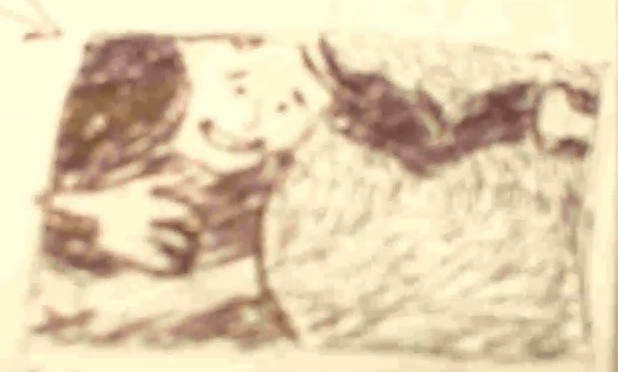
\includegraphics[width=0.25\textwidth]{./rysunki/fa.png}
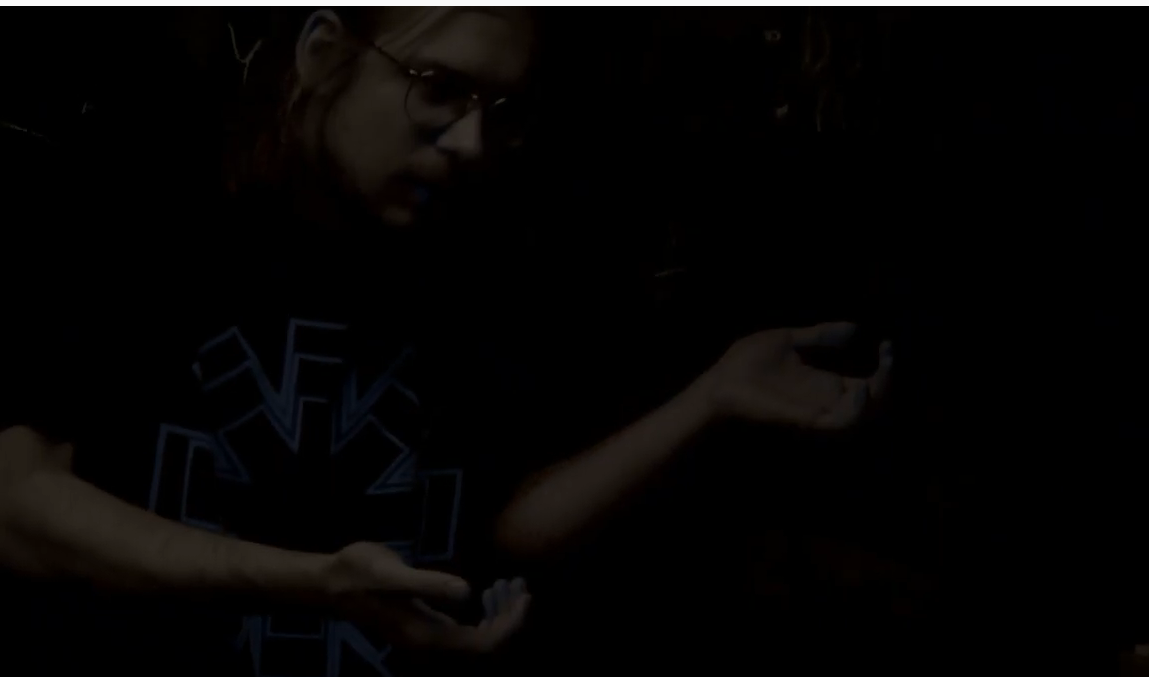
\includegraphics[width=0.25\textwidth]{./rysunki/ja/niebiesko.png}
% \includegraphics[width=0.25\textwidth]{./rysunki/ja/1.jpg}
% \includegraphics[width=0.25\textwidth]{./rysunki/ja/1.jpg}

\section{Uwaga o topologii}
Na zbiorze figur takich jak omawiane w tej pracy, branych z dokładnością do przesunięć i obrotów na
płaszczyźnie można określić odległość między nimi jako infimum pola sumy rozłącznej brane po wszystkich
reprezentantach klas (czyli po wszystkich obrazach izometrii na płaszczyźnie). \\
Czy to jest rzeczywiście matryka? \\
Tak, jest. \\
\begin{proof}
    1. $d(f,g) = 0 \iff f \cong g$. Implikacja w lewą stronę jest oczywista. Implikacja w prawą stronę,
    wynika z tego, że ze zwartości jeśli punkt należy do sumy rozłącznej, to należy wraz ze swoim otoczeniem,
     więc pole sumy rozłącznej jest >0. (Gdyby nie należał wraz z żdnym otoczeniem, to dowolnie blisko
     mógłbym podejść punktami z drugiej figury i z domkniętości tenże punkt też by należał). \\
     2. $d(f,g ) = d(g,f)$. Jest tak, bo różnicasymetryczna jest symetryczna. \\
     3. warunek trójkąta. Jest tak, bo odległość zdefiniowaliśmy przez infimum. (Serio wyszło
     \smalltodoII{napisać to}. \\

\end{proof}
Zauważmy, ż jeśli $\mathcal{P}(f)$ to pole figury $f$, to
\begin{equation}
    |\mathcal{P}(f) - \mathcal{P}(g)| \leq d(f, g)
\end{equation}
Wynika stąd, że dla dowolnej liczby rzeczywistej $r$, zbiór figur o polu $r$ jest zbiorem domkniętym.
(Nazwijmy ten zbiór $R$. Weźmy punkt $s$ spoza tego zbioru, niech ma on pole $m$.
Stąd $s$ jest w odległości co najmniej $|m-r|$ od każdego punktu z $R$. \\
Otoczenie będące kulą wokół $s$ o promieniu ostro mniejszym niż $|m - r|$ zawiera się więc w dopełnieniu $R$.
 Stąd dopełnienie $R$ jest otwarte, stąd $R$ jest domknięty. $_\square$)
\\
% Można zauważyć że zbiór figur o równym polu jest
%może jakiś ilozyn sklalarny
Można teraz zauważyć że w tak zdefiniowanej topologii na figurach każda klasa wyznaczona przez jeden z
elementów WGA (czyli klasa równoważności przez cięcia z zaniedbaniem zachowywania pola) jest zbiorem gęstym.
\\
% Dalej, można zawuważyć, że dla dowolnej takiej klasy, wystarczy ograniczyć się do figur, gdzie końce
% $C^\infty$ fragmentów leżą w punktach wymiernych.
Można też zauważyć, że skoro każdą figurę jestem w stanie dowolnie przybliżyć wielokątami o wierzchołkach
w punktach wymiernych, to powstała przestrzeń jest przestrzenią ośrodkową.
\\
% Dlaje można zauważyć, że każdy ciąg cauchyego w tej przestrzeni ma granicę. Stąd powstała przestrzeń figur
% jest przestrzenią polską. \\
Przestrzeń ta nie jest jednak zupełna. Jeżeli brzegi figur z ciągu zbiegając punktowo do jakieś ustalonej
figury, być może szerszej klasy (na przykłąd o brzegach będących krzywymi Jordana), to figury te
tworzą ciąg Cauchyego w opisanej wyżej przestrzeni. Granica ciągu krzywych takich jak tu rozważanych nie musi
 być jednak głądką krzywą.
% Każda klasa równoważności przez cięcia (z zachowaniem pola) jest za to zbiorem gęstym w zbiorze domkniętym
% (figur o danym polu). \\
% % Dlaje można zauważyć, że każdy ciąg cauchyego w tej przestrzeni ma granicę. Stąd powstała przestrzeń figur
% % jest przestrzenią polską. \\
% % Teraz przystąpimy do wyznaczenia klasy zlożoności klasy podziału figury przez cięcia. \\
%
% \begin{proof}
%
% \end{proof}
%
\end{document}
